\documentclass[11pt,letterpaper]{article}
\usepackage{fullpage}

\usepackage[english]{babel}
\usepackage[utf8]{inputenc}
\usepackage{amsmath}
\usepackage{graphicx}
\usepackage[hidelinks]{hyperref}
\usepackage{float}
\usepackage{amsfonts}
\usepackage{algorithm,algpseudocode}
             
\graphicspath{{../results}}
             
\begin{document} 

\title{Experiment 1}
\maketitle

\section*{Simulation Details}

Considered $K = 3$, $T = 5005$, $N = 125$. Report statistics at $t = 1000, 3000, 5000$ \\
\textbf{The Bandit priors that were considered}:
\begin{itemize}
\item Uniform: Draw the mean rewards for the arms from [0.25, 0.75]
\item ``HeavyTail": We took the mean rewards to be randomly drawn from Beta($\alpha=0.6,\beta=0.6$). With this distribution it was likely to have arms that were at the extremes (close to 1 and close to 0) but also some of the arms with intermediate value means.
\item Needle-in-haystack
\begin{enumerate}
\item Medium - 9 arms with mean 0.50, 1 arm with mean 0.55 (+ 0.05)
\item High - 9 arms with mean 0.50, 1 arm with mean 0.70 (+ 0.20)
\end{enumerate}
\end{itemize}
\textbf{Algorithms considered}:
\begin{enumerate}
\item ThompsonSampling with priors of $Beta(1, 1)$ for every arm.
\item DynamicGreedy with priors of $Beta(1, 1)$ for every arm
\item Bayesian Dynamic $\epsilon$-greedy with priors of $Beta(1, 1)$ for every arm and $\epsilon=0.05$
\end{enumerate}
\textbf{Agent Algorithms considered}:
\begin{enumerate}
\item HardMax
\item HardMaxWithRandom
\item SoftMax
\end{enumerate}
\textbf{Memory Sizes}
\begin{enumerate}
\item 10
\item 25
\item 100
\end{enumerate}
\pagebreak
\textbf{Simulation Procedure}
\begin{algorithm}
\begin{algorithmic}[1]
\For{Each prior $p$}
	\For{Each agent algorithm $agent alg$}
		\For{Each principal algorithm pair $principalalg1$, $principalalg2$}
			\For{$N$ simulations}
				\State Generate true distribution from $p$ (except for needle-in-		haystack, just use $p$ itself)
				\State Run simulation for T periods
			\EndFor
		\EndFor
	\EndFor
\EndFor
\end{algorithmic}
\end{algorithm}

\pagebreak
\section*{Results}

One thing which is ambiguous to define is the regret value to use when a principal never gets chosen in a given simulation. When calculating any of the aggregate regret statistics we drop these simulations, but we do record how many rounds have an undefined regret. \\
\vspace{1cm}

First, we'll restrict focus to $t = 5000$ and look at the performance of ThompsonSampling. Note that the y axis here represents the market share that the ThompsonSampling principal gets.
\vspace{0.5cm}
Performance of ThompsonSampling vs DynamicGreedy and DynamicEpsilonGreedy across all agent models, memory sizes, and priors: \\
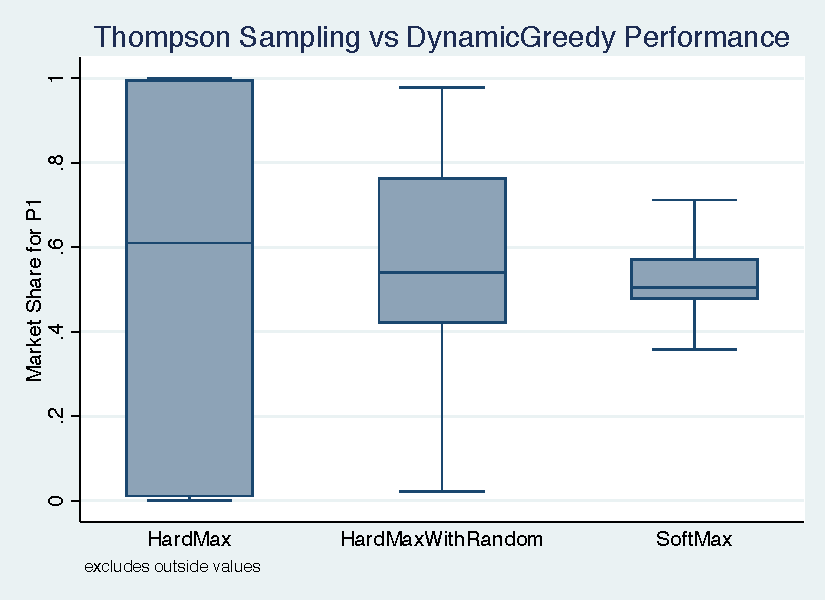
\includegraphics[scale=0.75]{ts_perf_dg} \\
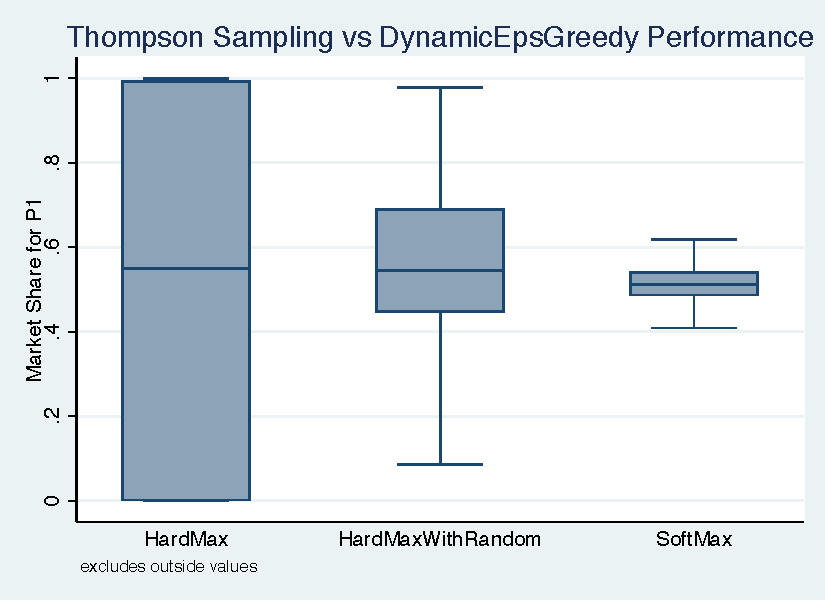
\includegraphics[scale=0.75]{ts_perf_deg} \\

Now, looking across different memory sizes for each agent model (still using each prior): \\
\textbf{HardMax} \\
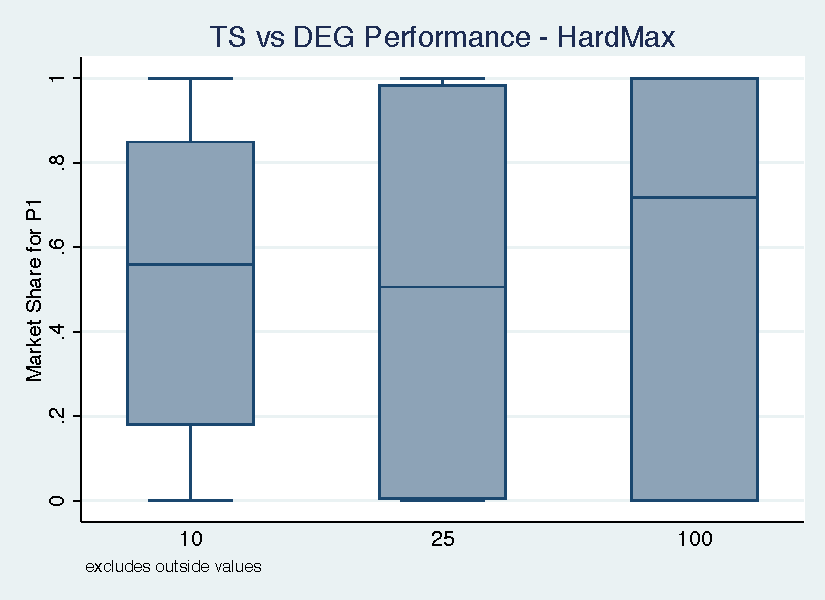
\includegraphics[scale=1]{hm_ts_deg} \\
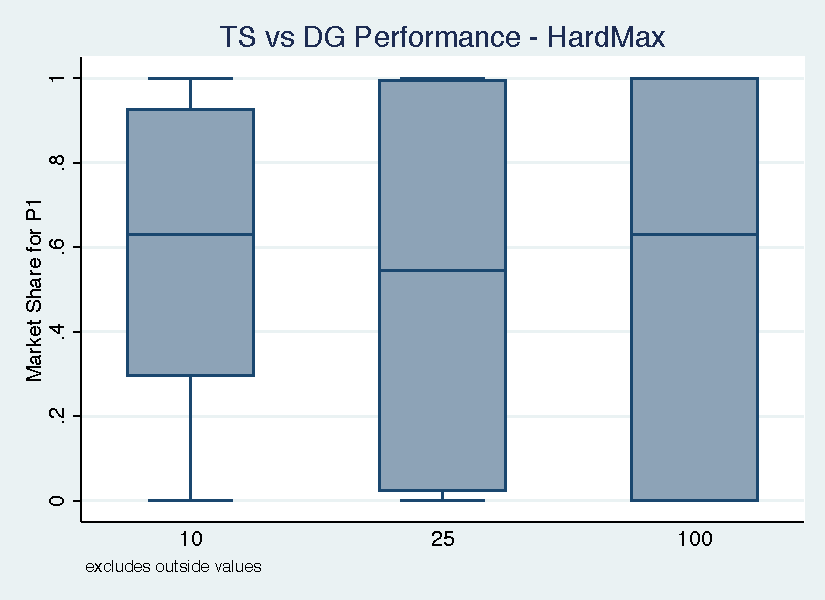
\includegraphics[scale=1]{hm_ts_dg}

\pagebreak
\textbf{HardMaxWithRandom} \\
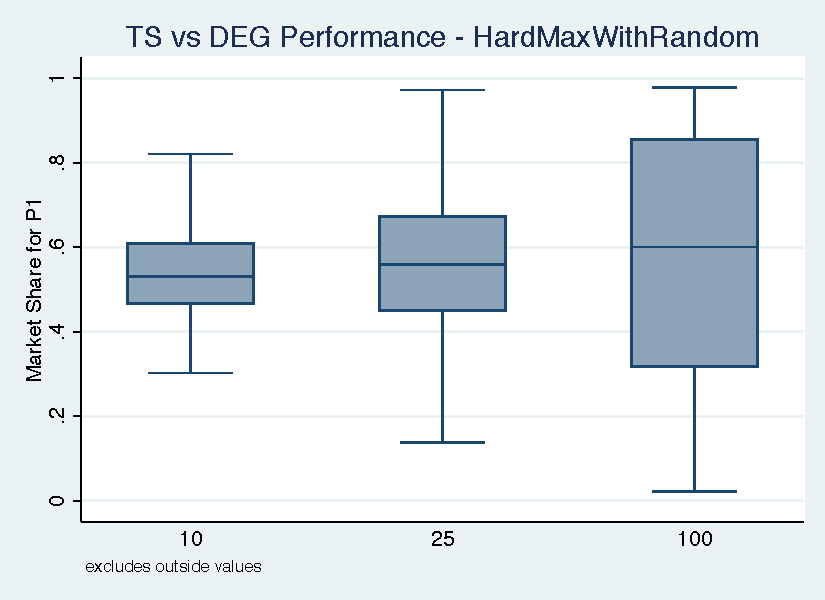
\includegraphics[scale=1]{hmr_ts_deg} \\
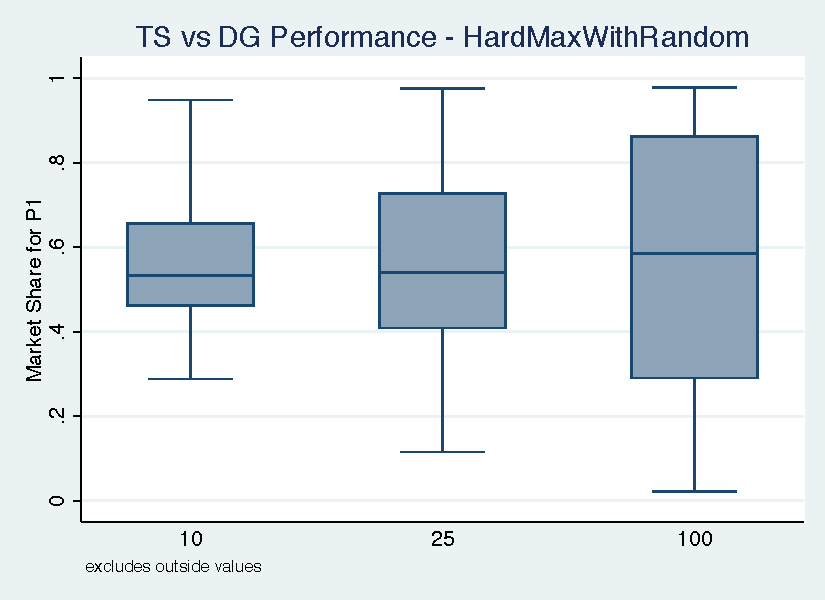
\includegraphics[scale=1]{hmr_ts_dg}

\pagebreak
\textbf{SoftMax} \\
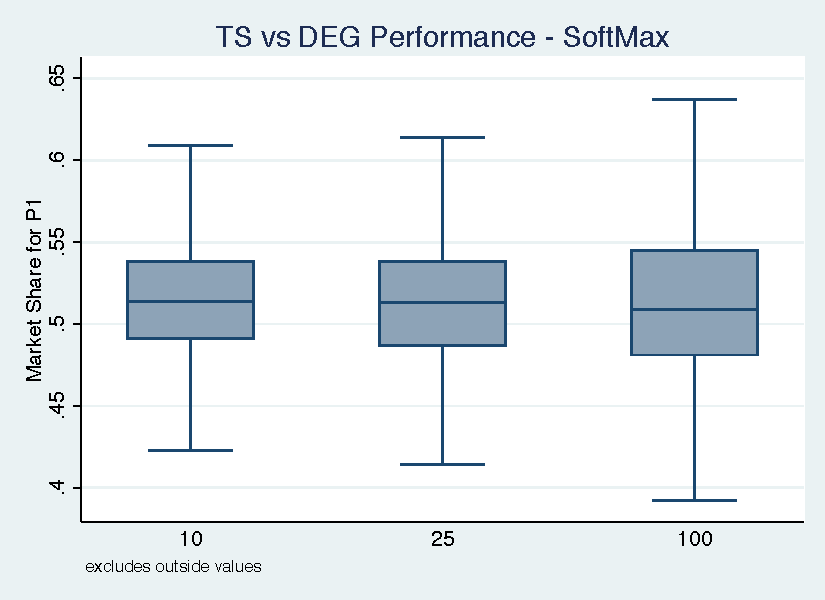
\includegraphics[scale=1]{sm_ts_deg} \\
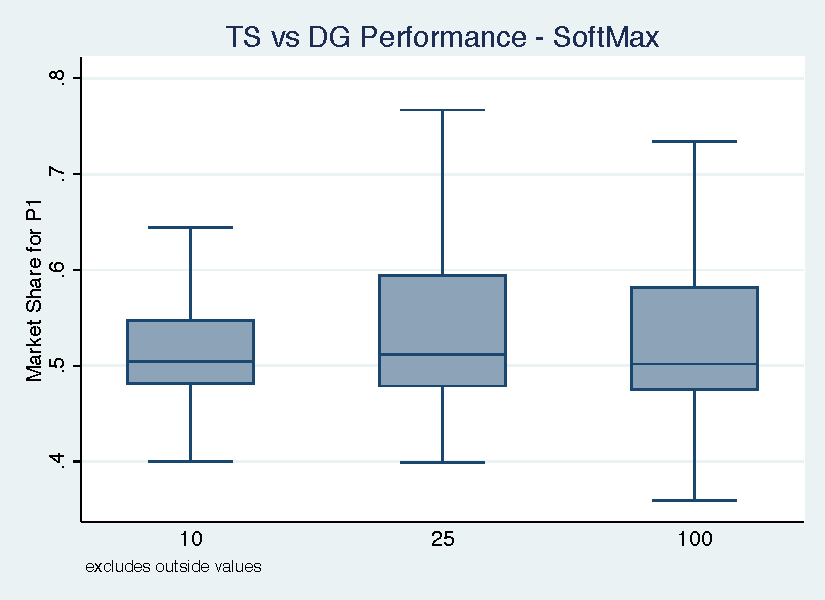
\includegraphics[scale=1]{sm_ts_dg}

\pagebreak
We'll now look fix memory size to be 100 and look at the performance across priors.\\
\textbf{HardMax} \\
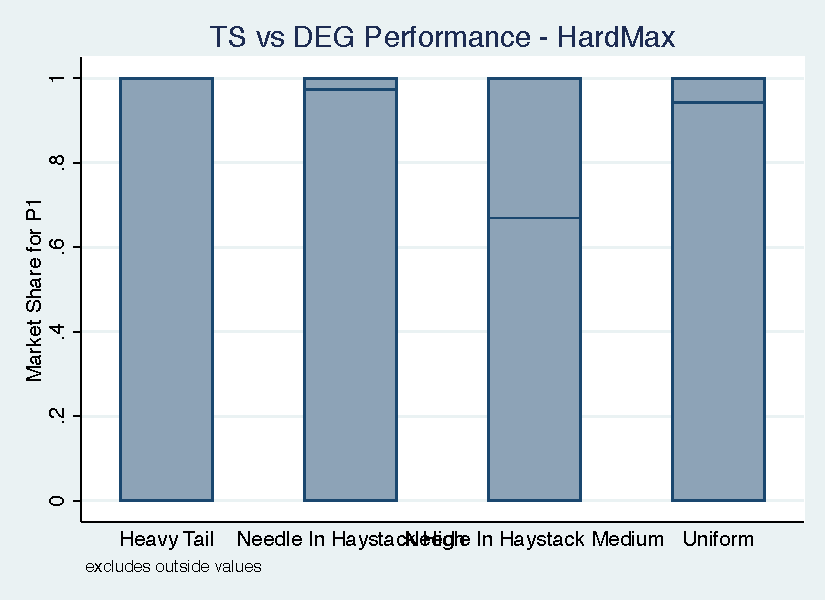
\includegraphics[scale=1]{hm_ts_deg_prior} \\
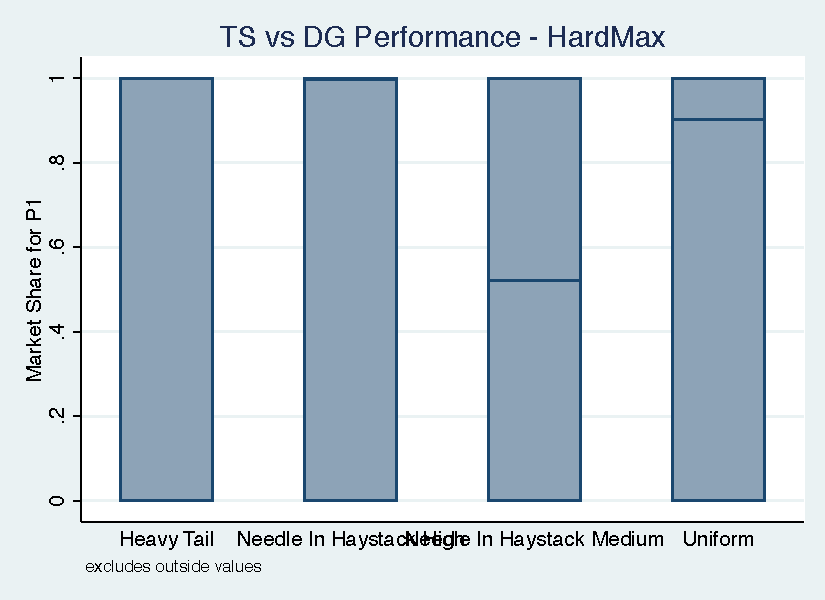
\includegraphics[scale=1]{hm_ts_dg_prior}

\pagebreak
\textbf{HardMaxWithRandom} \\
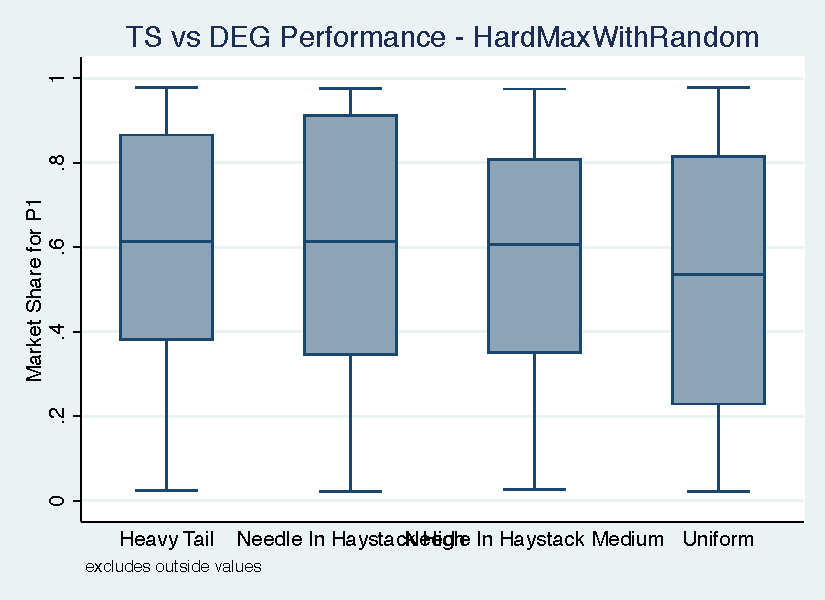
\includegraphics[scale=1]{hmr_ts_deg_prior} \\
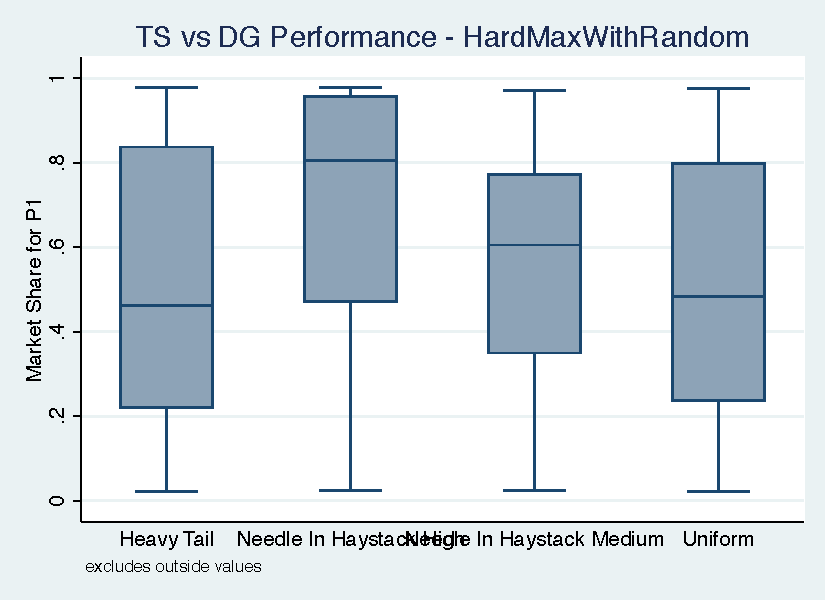
\includegraphics[scale=1]{hmr_ts_dg_prior}

\pagebreak
\textbf{SoftMax} \\
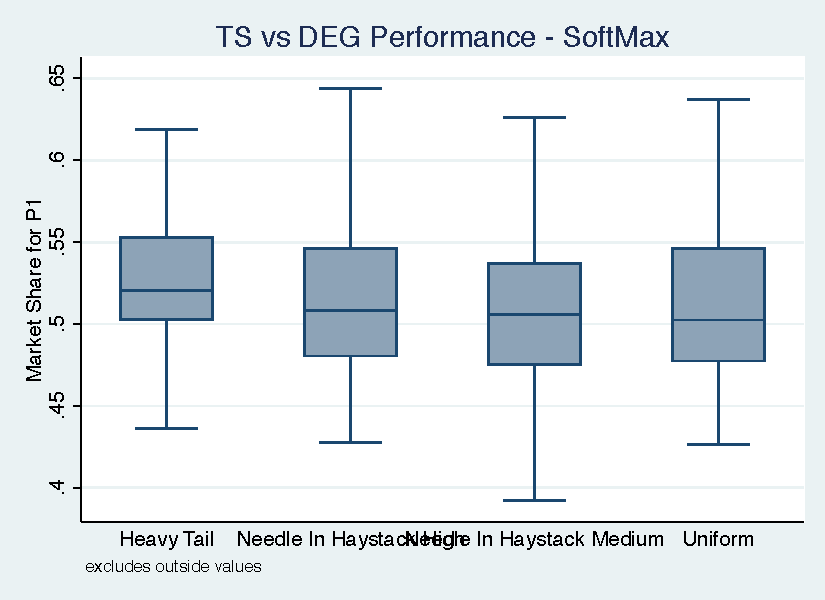
\includegraphics[scale=1]{sm_ts_deg_prior} \\
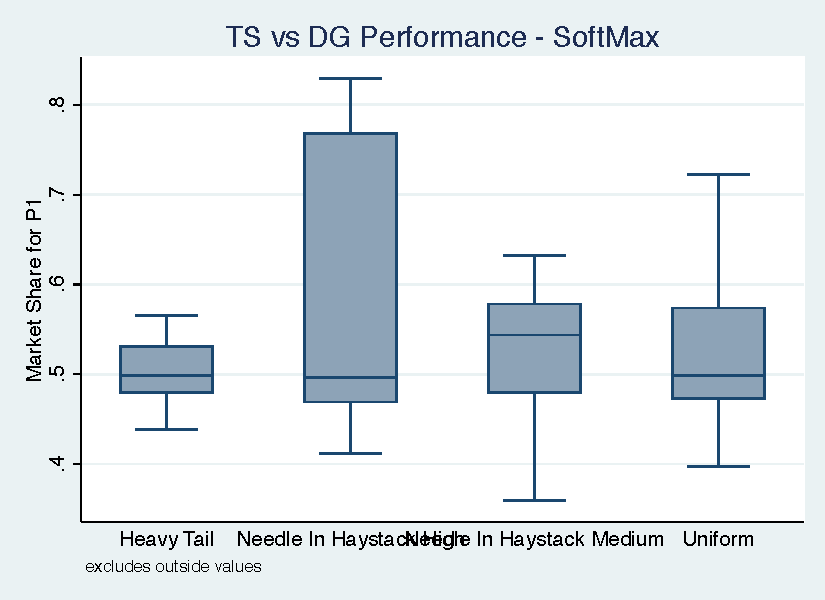
\includegraphics[scale=1]{sm_ts_dg_prior}



\end{document}